%%%%%%%%%%%%%%%%%%%%%%%%%%%%%%%%%%%%%%%%%%%%%%%%%%%%%%%
\begin{frame}

\frametitle{Overview}

Snakemake is:
\begin{itemize}
  \item A {\red{workflow}} definition language, similar to Make.
  \item Based on {\green{Python}}.
  \item Developed for bioinformatics\footnote{The application of computer science, statistics, etc. to problems in the life sciences.}, but general enough for other tasks.
\end{itemize}

\end{frame}


%%%%%%%%%%%%%%%%%%%%%%%%%%%%%%%%%%%%%%%%%%%%%%%%%%%%%%%
\begin{frame}

\frametitle{Disclaimer}

\begin{quotation}
In terms of scripts, I'm primarily a Perl programmer and have had to learn Python the past year because of Snakemake.  Thus, I don't claim to be an expert of either Python or Snakemake.  I will cover what I've needed to know (so far).
\vs

Hopefully this talk will give you enough information to decide if Snakemake is useful for your work.
\end{quotation}

\end{frame}


%%%%%%%%%%%%%%%%%%%%%%%%%%%%%%%%%%%%%%%%%%%%%%%%%%%%%%%
\begin{frame}

\frametitle{Pipelines}

Like other areas of data analysis, bioinformaticians often chain a series of programs together so that the output of one program becomes the input of another:

\begin{figure}
  \centering
  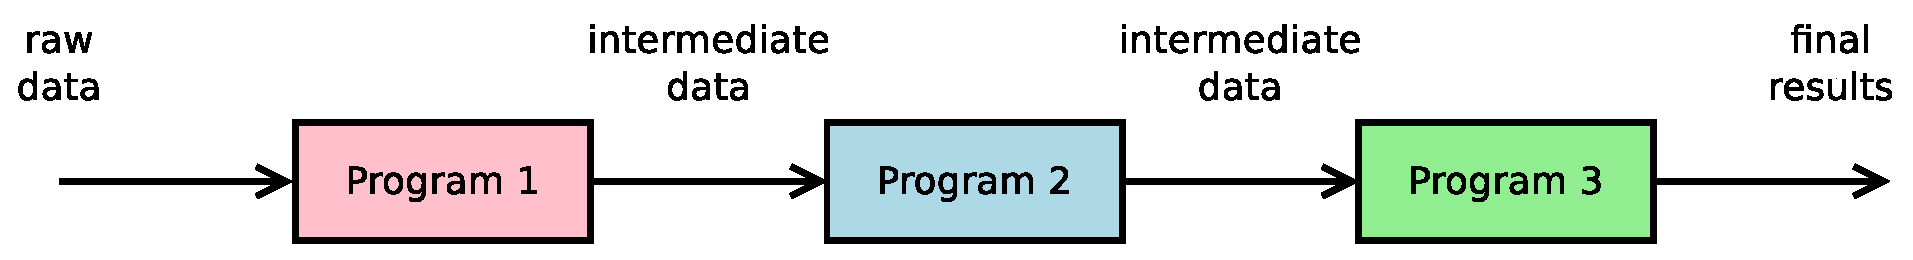
\includegraphics[width=\linewidth]{intro/pipeline-ex}
\end{figure}

\end{frame}


%%%%%%%%%%%%%%%%%%%%%%%%%%%%%%%%%%%%%%%%%%%%%%%%%%%%%%%
\begin{frame}[fragile]

\frametitle{Make}

For longer than what some of us are willing to admit \smiley, we may have used Make to build programs and libraries from source code.\\
\vs

Files with the filename {\texttt{Makefile}} are used with rules of this form:

\begin{figure}
  \centering
\begin{lstlisting}[language=make]
target:  dependencies
    system command(s)
\end{lstlisting}
\end{figure}

\end{frame}


%%%%%%%%%%%%%%%%%%%%%%%%%%%%%%%%%%%%%%%%%%%%%%%%%%%%%%%
\begin{frame}[fragile]

\frametitle{Make}

Thus, a rule in a Makefile might look like this:

\begin{figure}
  \centering
\begin{lstlisting}[language=make]
helloworld:  helloworld.c
	gcc helloworld.c -o helloworld
\end{lstlisting}
\end{figure}

When compiling a program with a Makefile, you might be using one compiler to compile source files to object files, linking them, and maybe even doing this in parallel.

\end{frame}


%%%%%%%%%%%%%%%%%%%%%%%%%%%%%%%%%%%%%%%%%%%%%%%%%%%%%%%
\begin{frame}

\frametitle{Galaxy}

Not surprisingly, bioinformaticians have developed their own systems (too numerous to list them all) which ultimately do almost the same thing (from a computing perspective).
\vs

Galaxy (which predates Snakemake) is a web-based system for constructing such workflows.

\end{frame}


%%%%%%%%%%%%%%%%%%%%%%%%%%%%%%%%%%%%%%%%%%%%%%%%%%%%%%%
\begin{frame}

\frametitle{Galaxy}

\begin{figure}
  \centering
  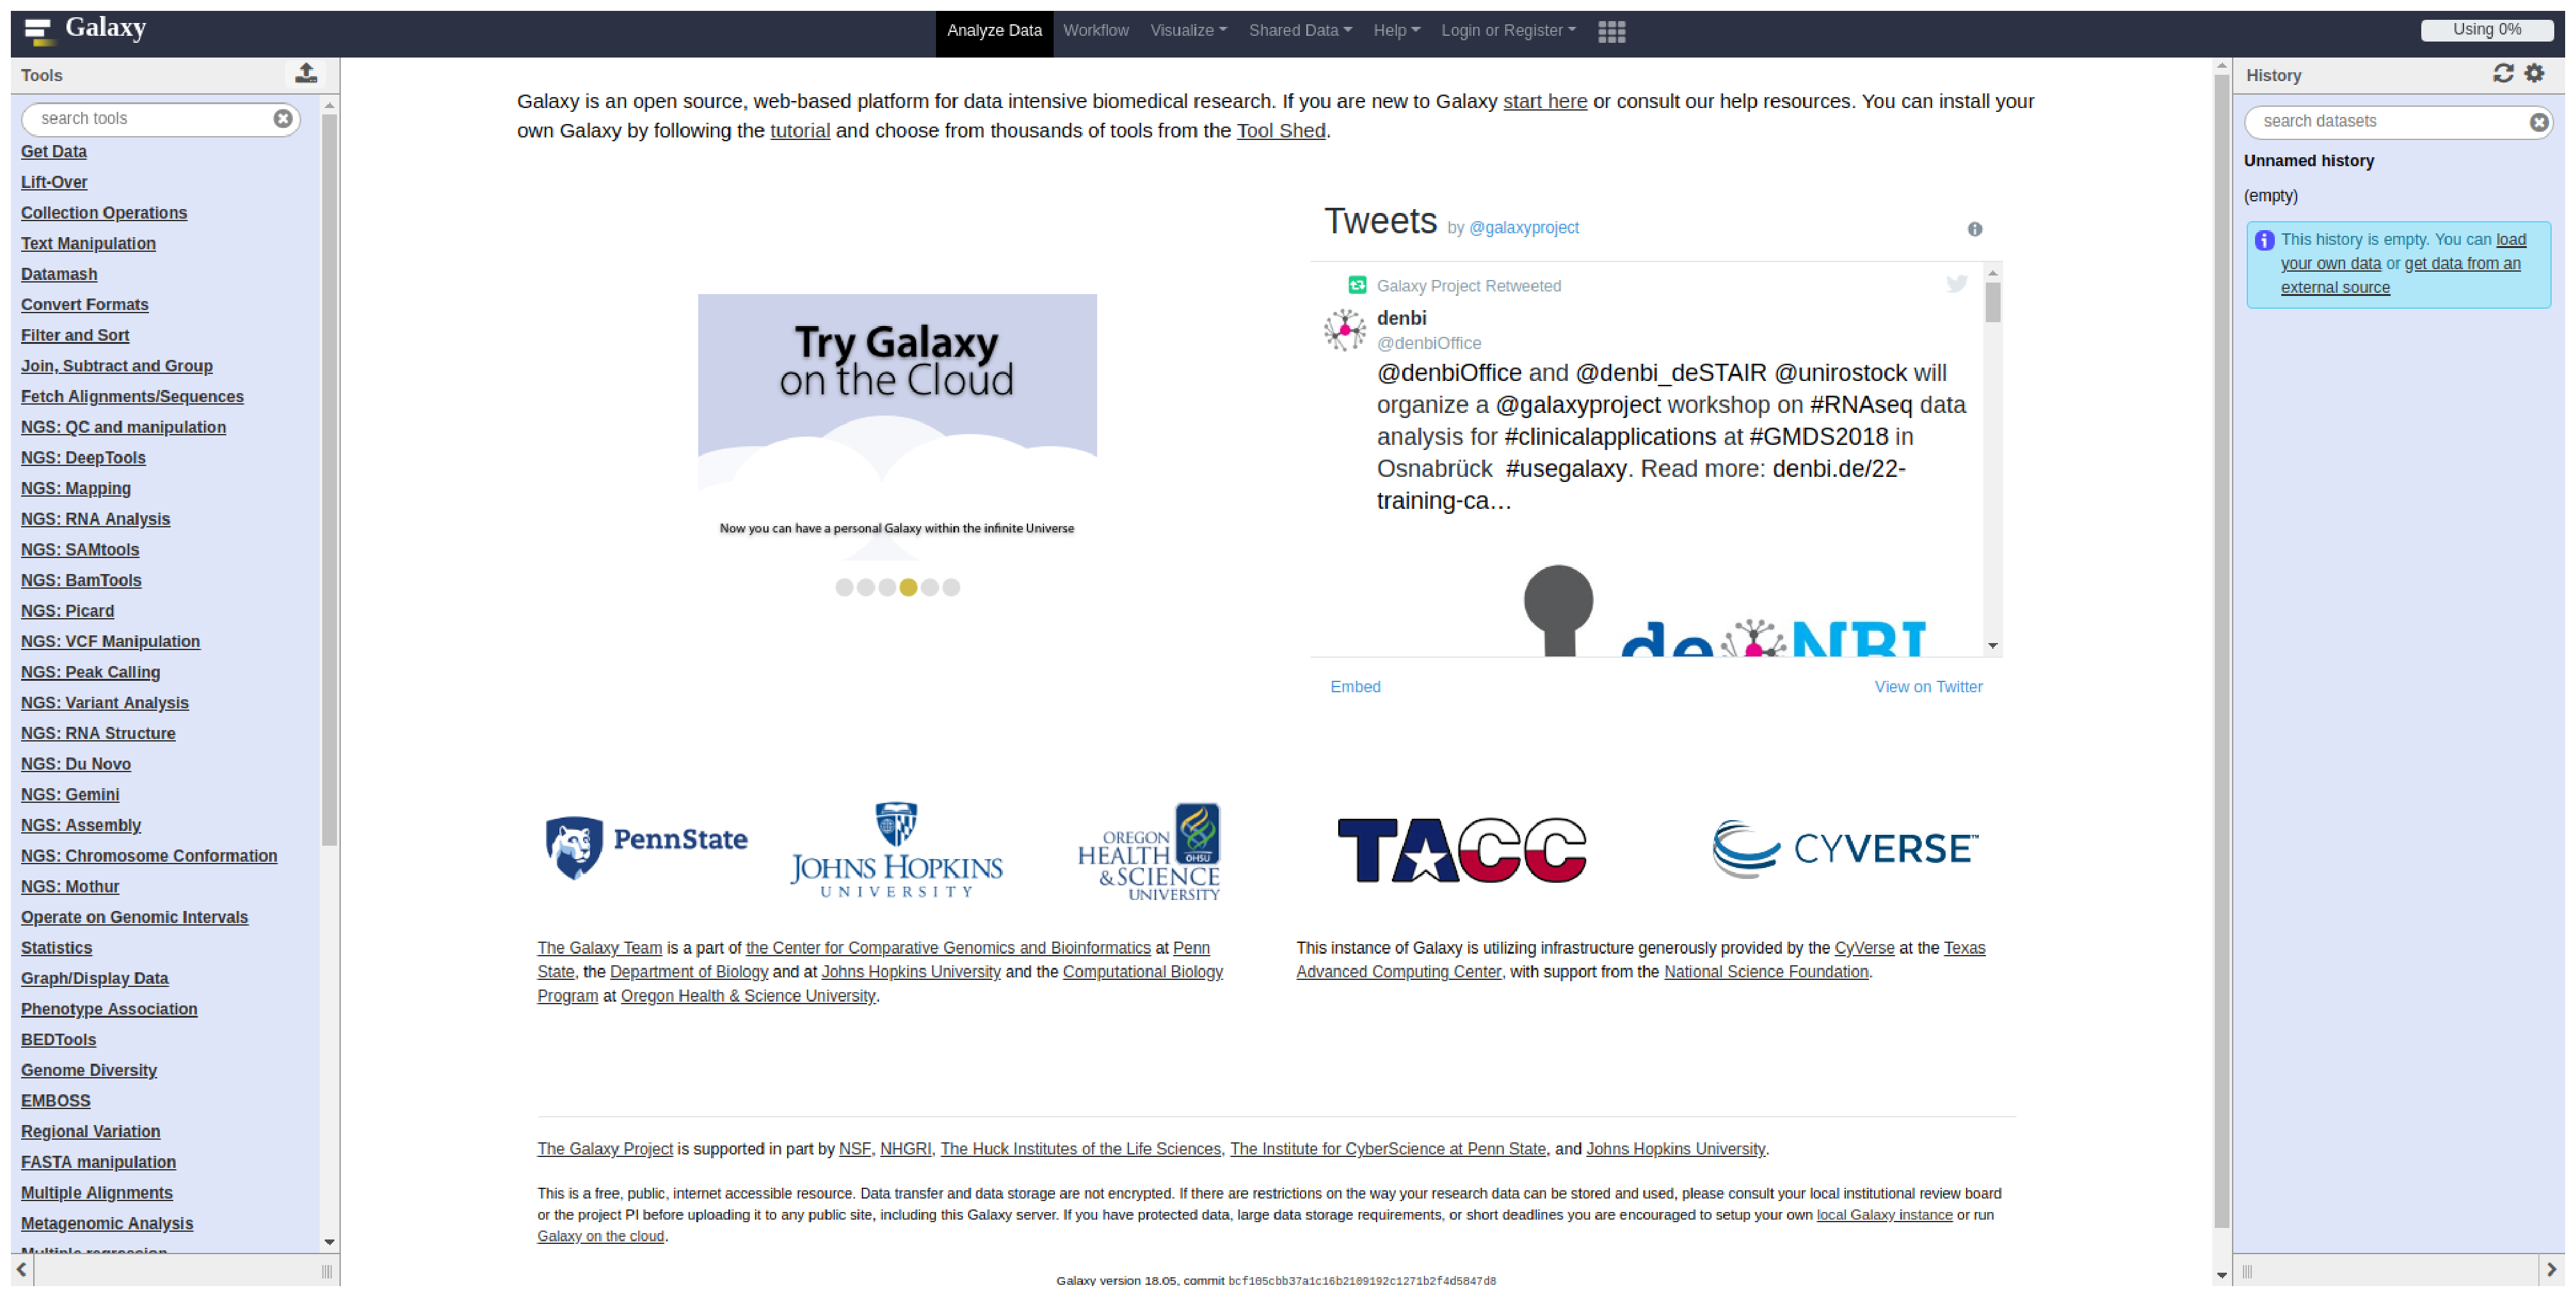
\includegraphics[width=\linewidth]{intro/galaxy-0}
\end{figure}

{\figsource{\href{https://usegalaxy.org/}{https://usegalaxy.org/}}}

\end{frame}


%%%%%%%%%%%%%%%%%%%%%%%%%%%%%%%%%%%%%%%%%%%%%%%%%%%%%%%
\begin{frame}

\frametitle{Galaxy}

\begin{figure}
  \centering
  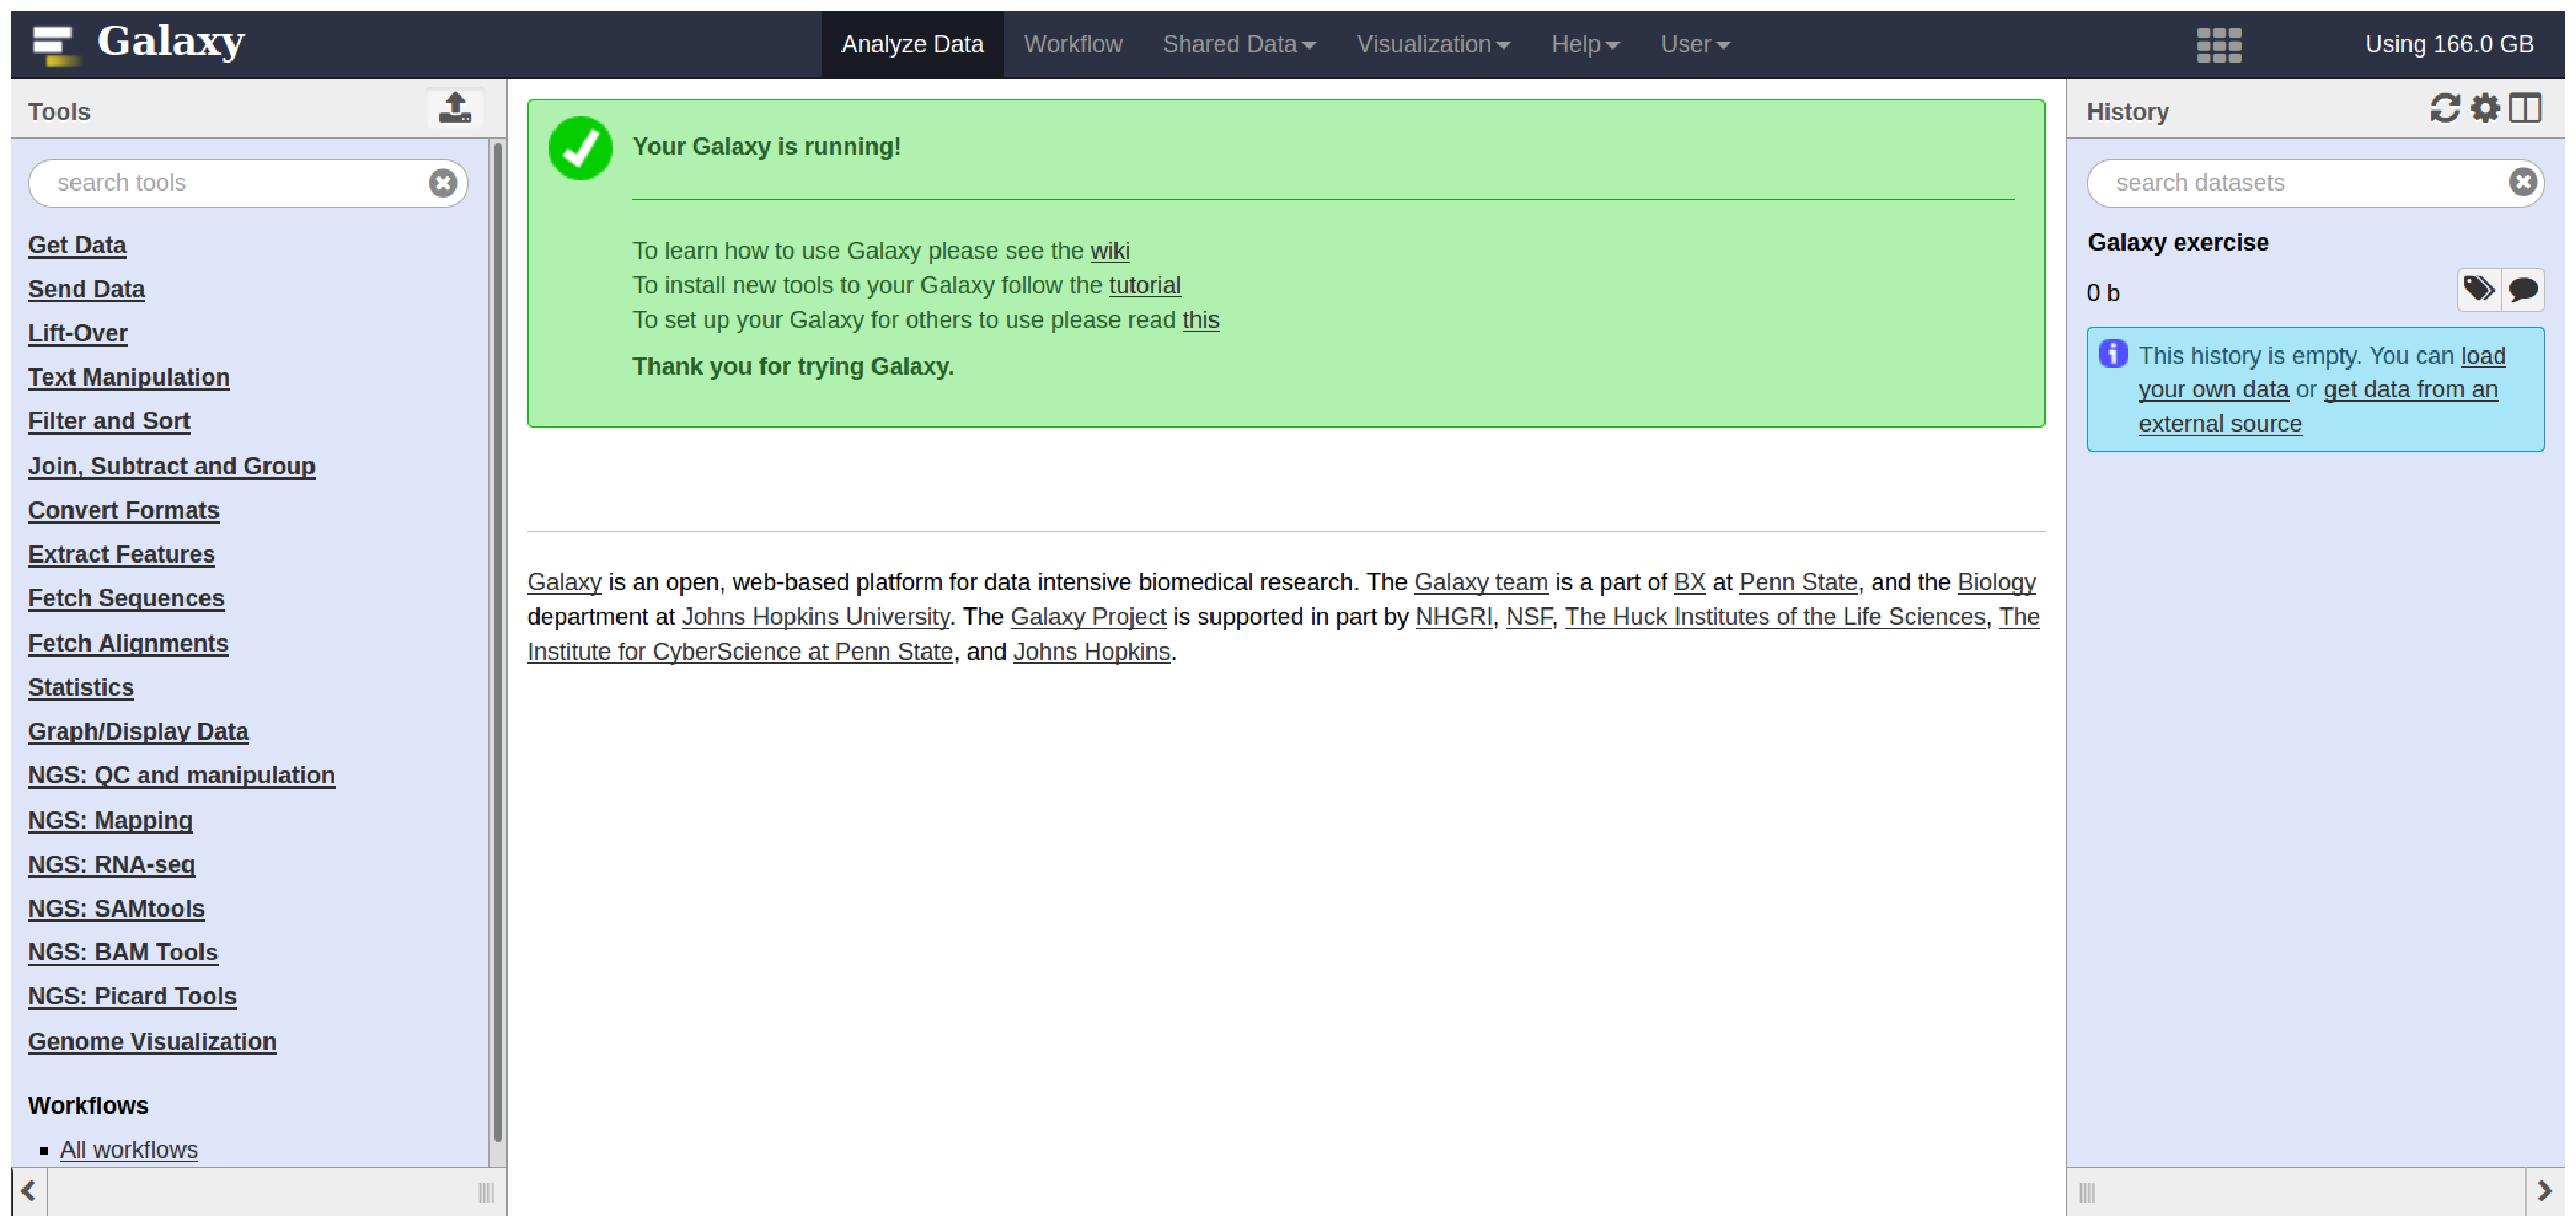
\includegraphics[width=\linewidth]{intro/galaxy-1}
\end{figure}

{\figsource{Local installation}}

\end{frame}


%%%%%%%%%%%%%%%%%%%%%%%%%%%%%%%%%%%%%%%%%%%%%%%%%%%%%%%
\begin{frame}

\frametitle{Galaxy}

\begin{figure}
  \centering
  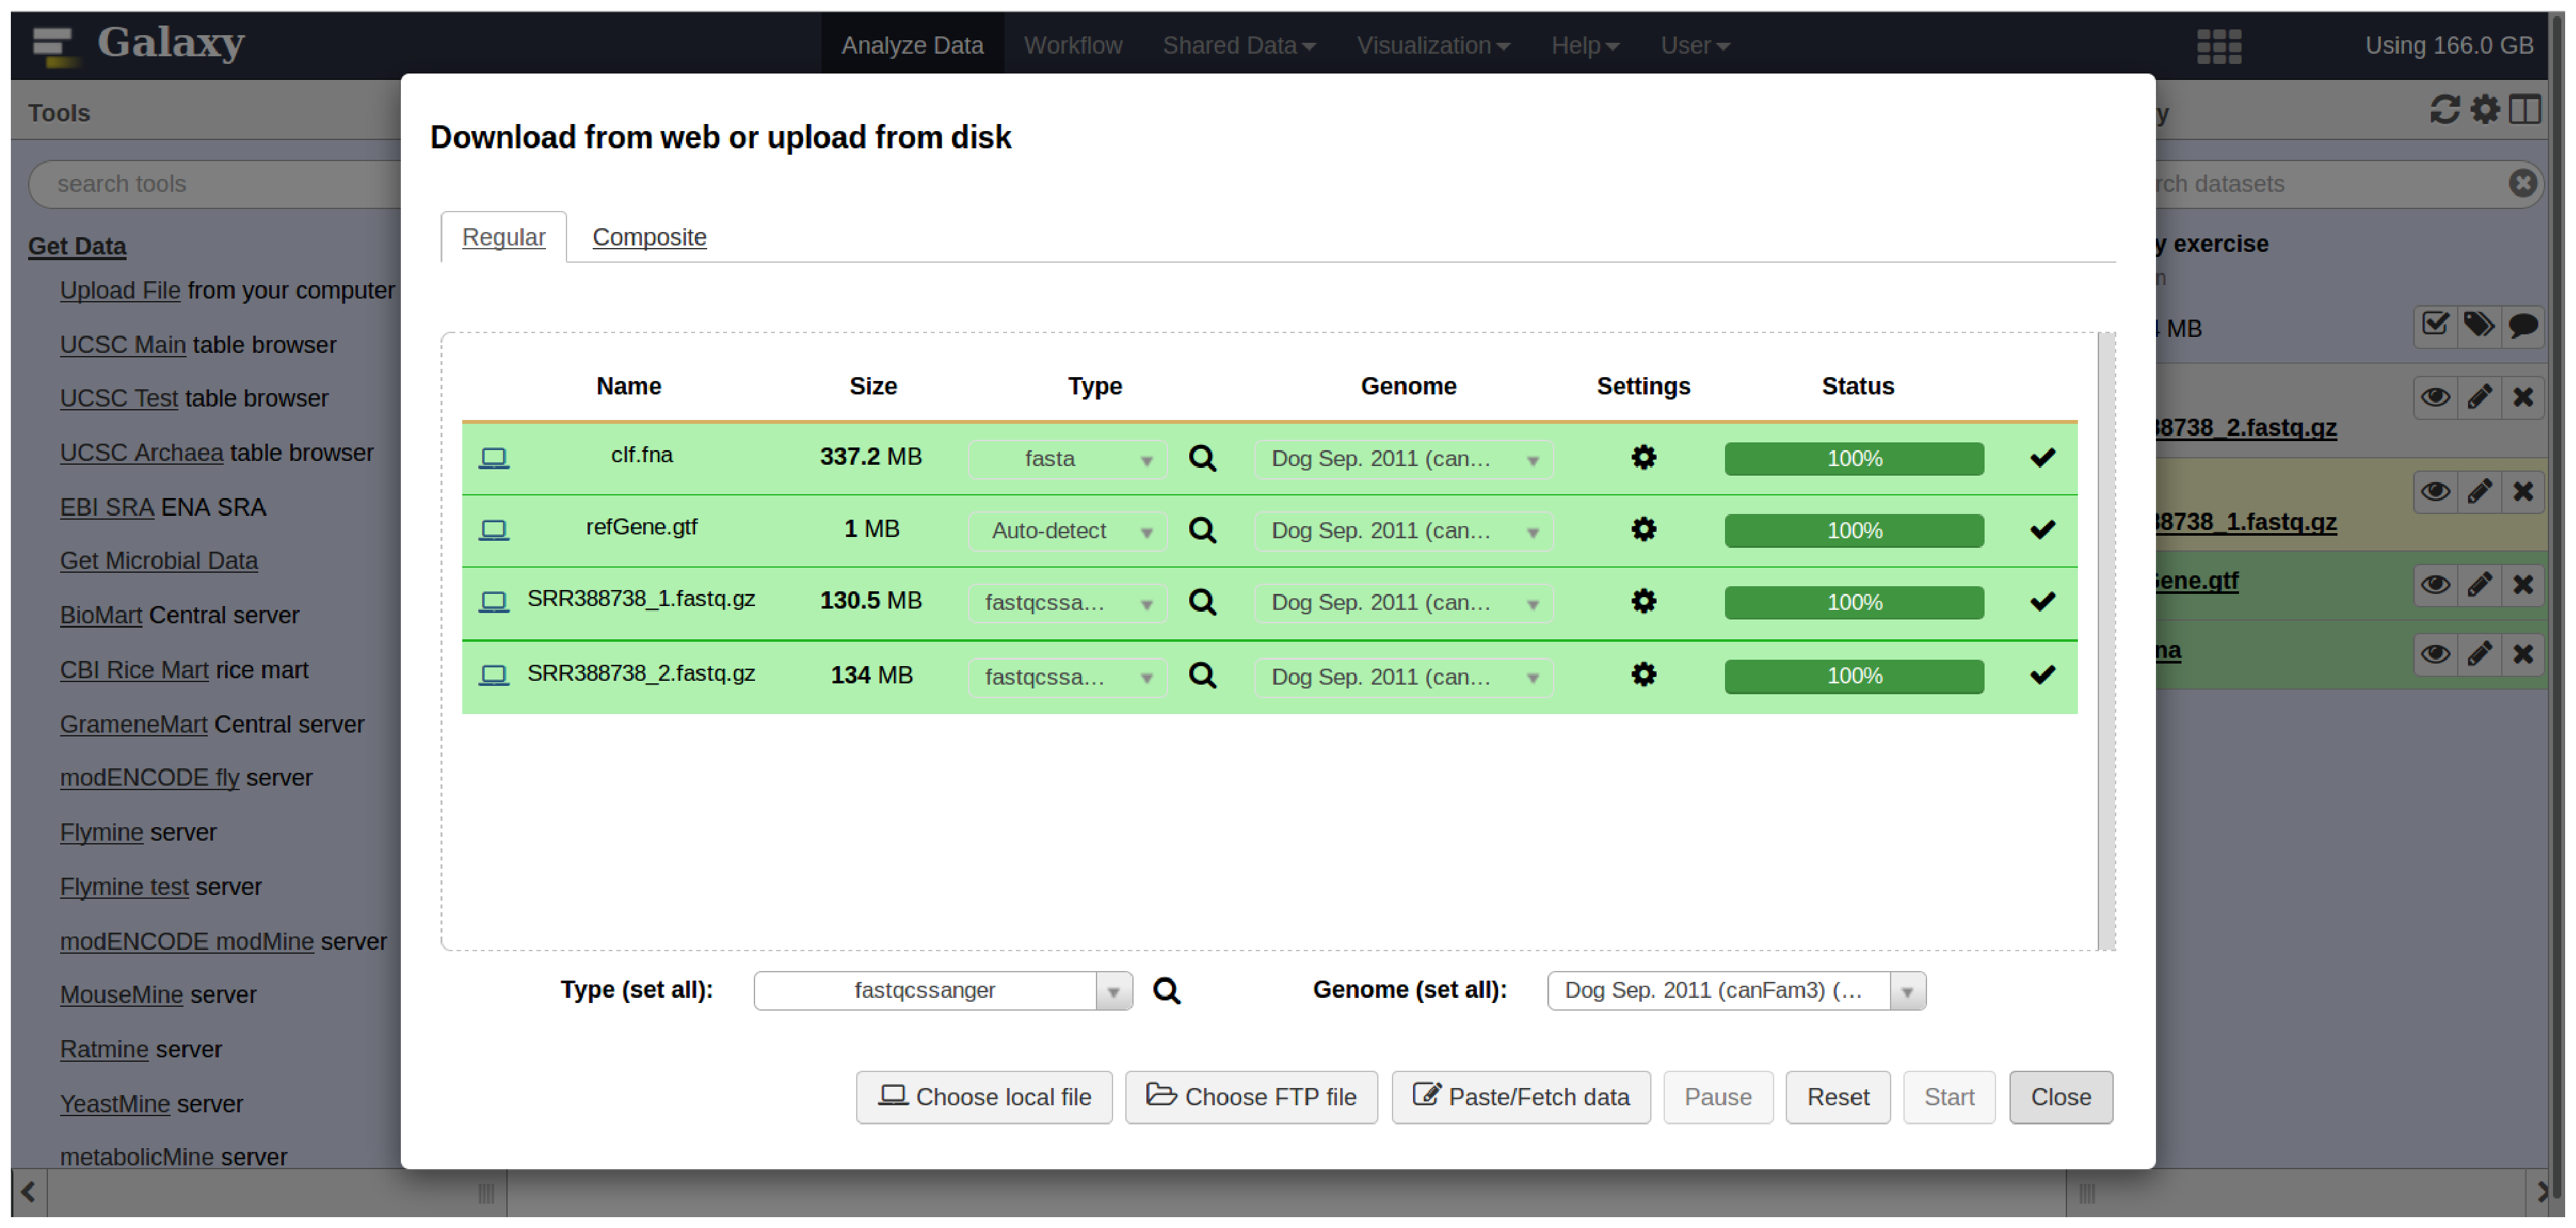
\includegraphics[width=\linewidth]{intro/galaxy-2}
\end{figure}

\end{frame}


%%%%%%%%%%%%%%%%%%%%%%%%%%%%%%%%%%%%%%%%%%%%%%%%%%%%%%%
\begin{frame}

\frametitle{Galaxy}

\begin{figure}
  \centering
  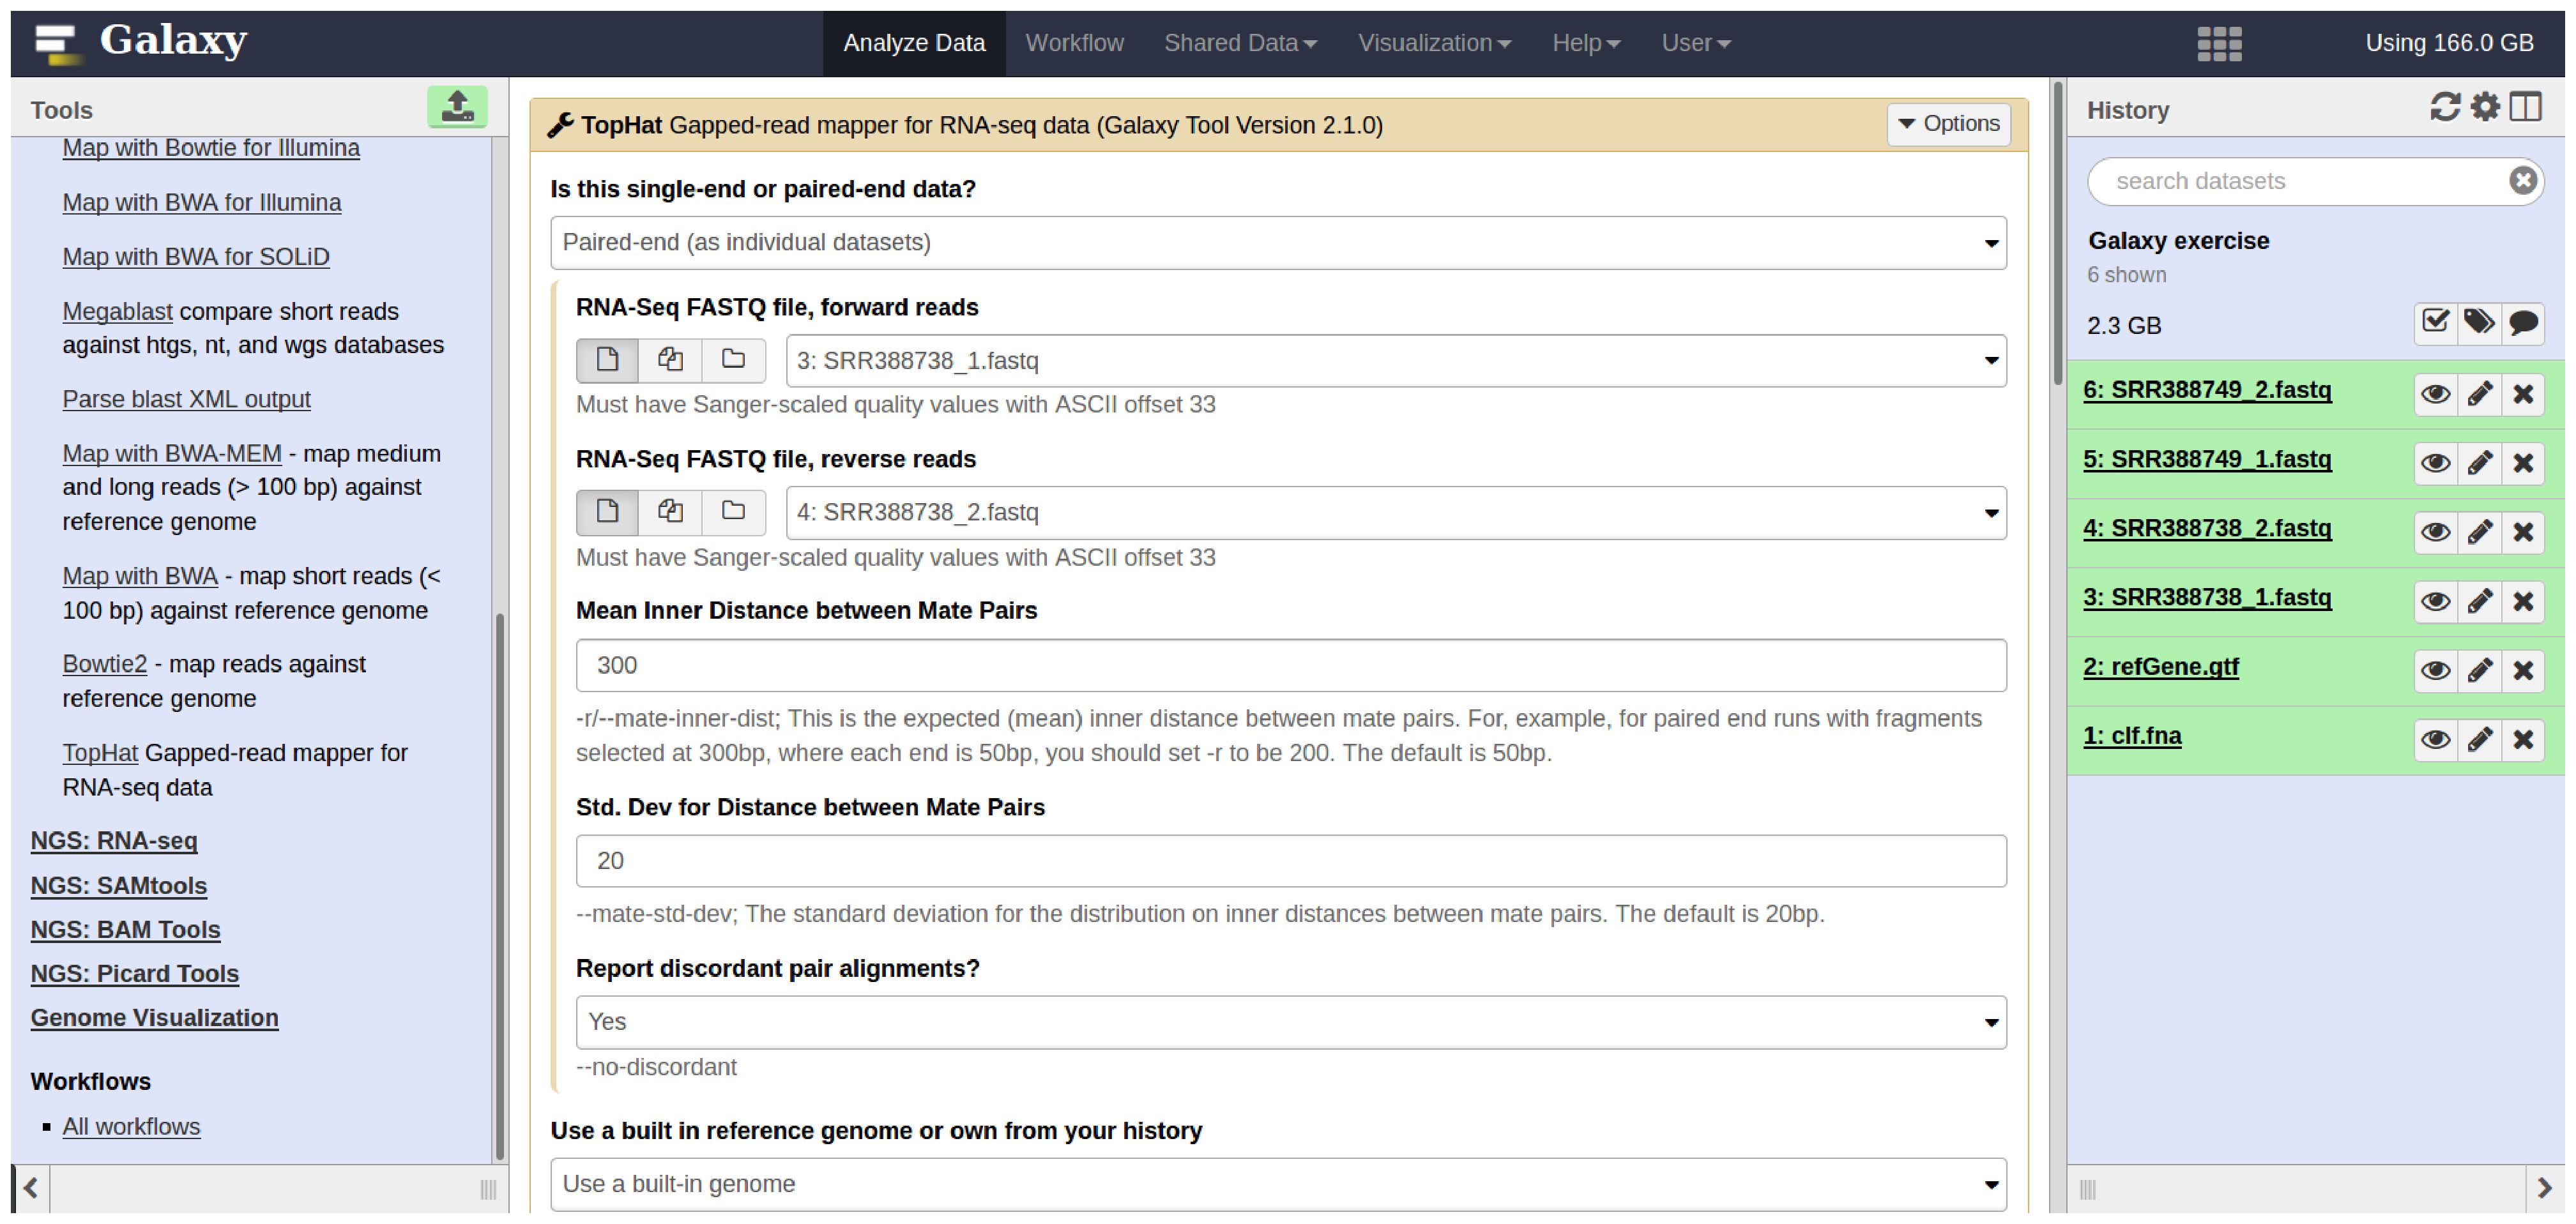
\includegraphics[width=\linewidth]{intro/galaxy-3}
\end{figure}

\end{frame}


%%%%%%%%%%%%%%%%%%%%%%%%%%%%%%%%%%%%%%%%%%%%%%%%%%%%%%%
\begin{frame}

\frametitle{Galaxy}

\begin{figure}
  \centering
  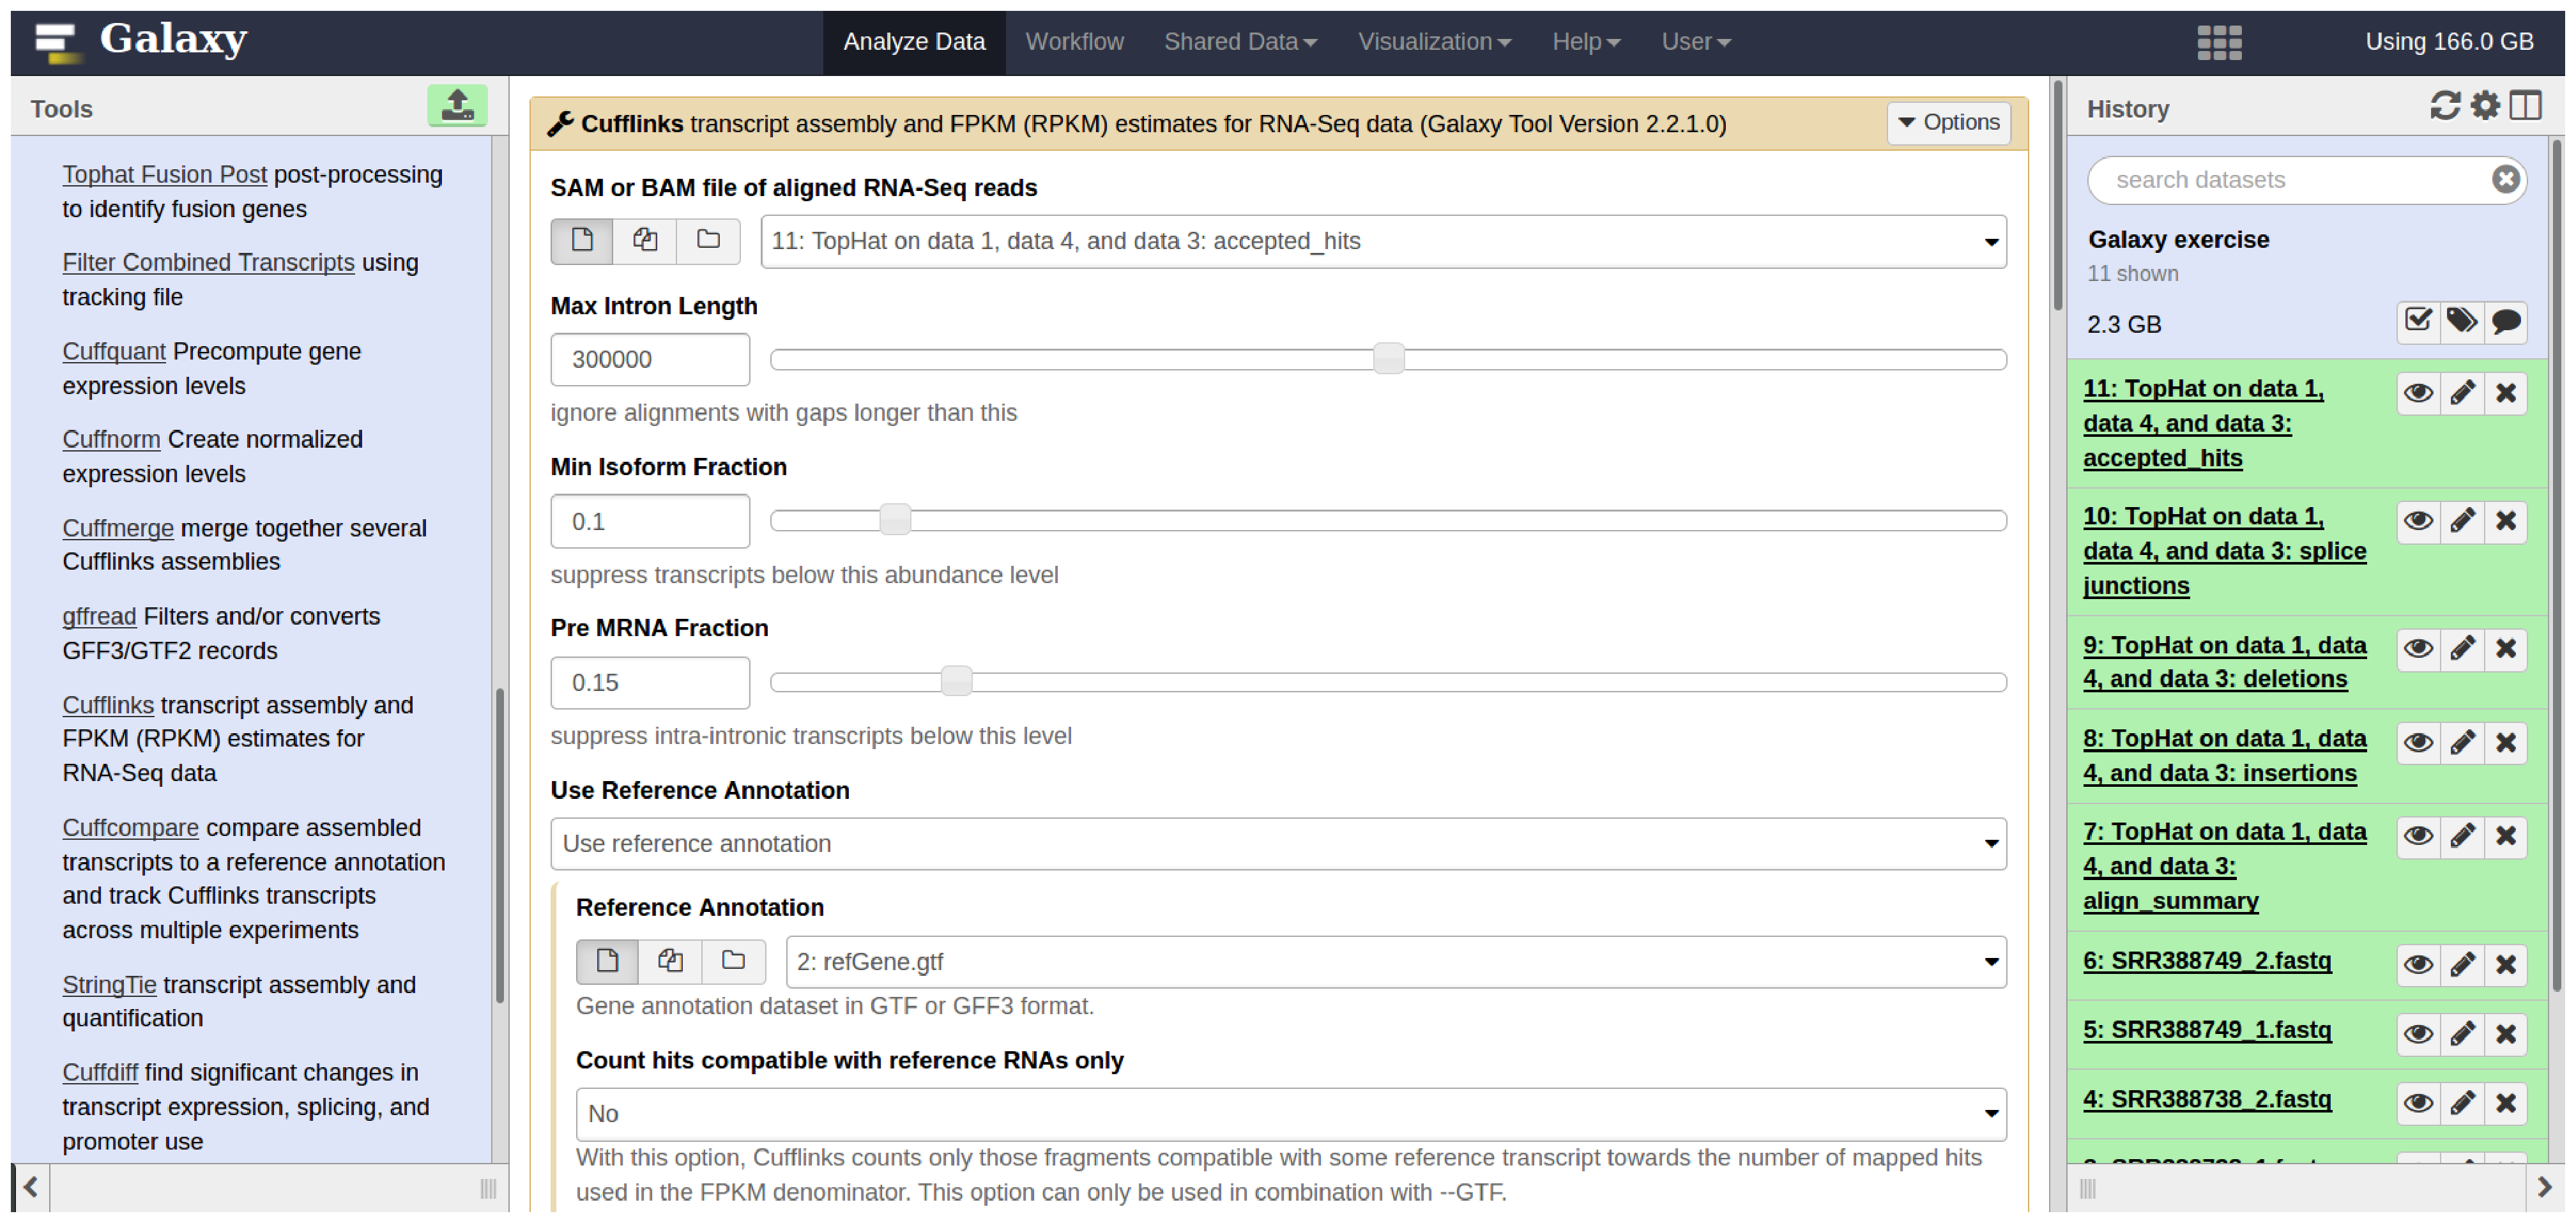
\includegraphics[width=\linewidth]{intro/galaxy-4}
\end{figure}

While it's conceivable to generalize Galaxy for non-bioinformaticians, it's probably not worth the effort...

\end{frame}


%%%%%%%%%%%%%%%%%%%%%%%%%%%%%%%%%%%%%%%%%%%%%%%%%%%%%%%
\begin{frame}

\frametitle{Snakemake}

Published in 2012 in the context of bioinformatics:

\begin{figure}
  \centering
  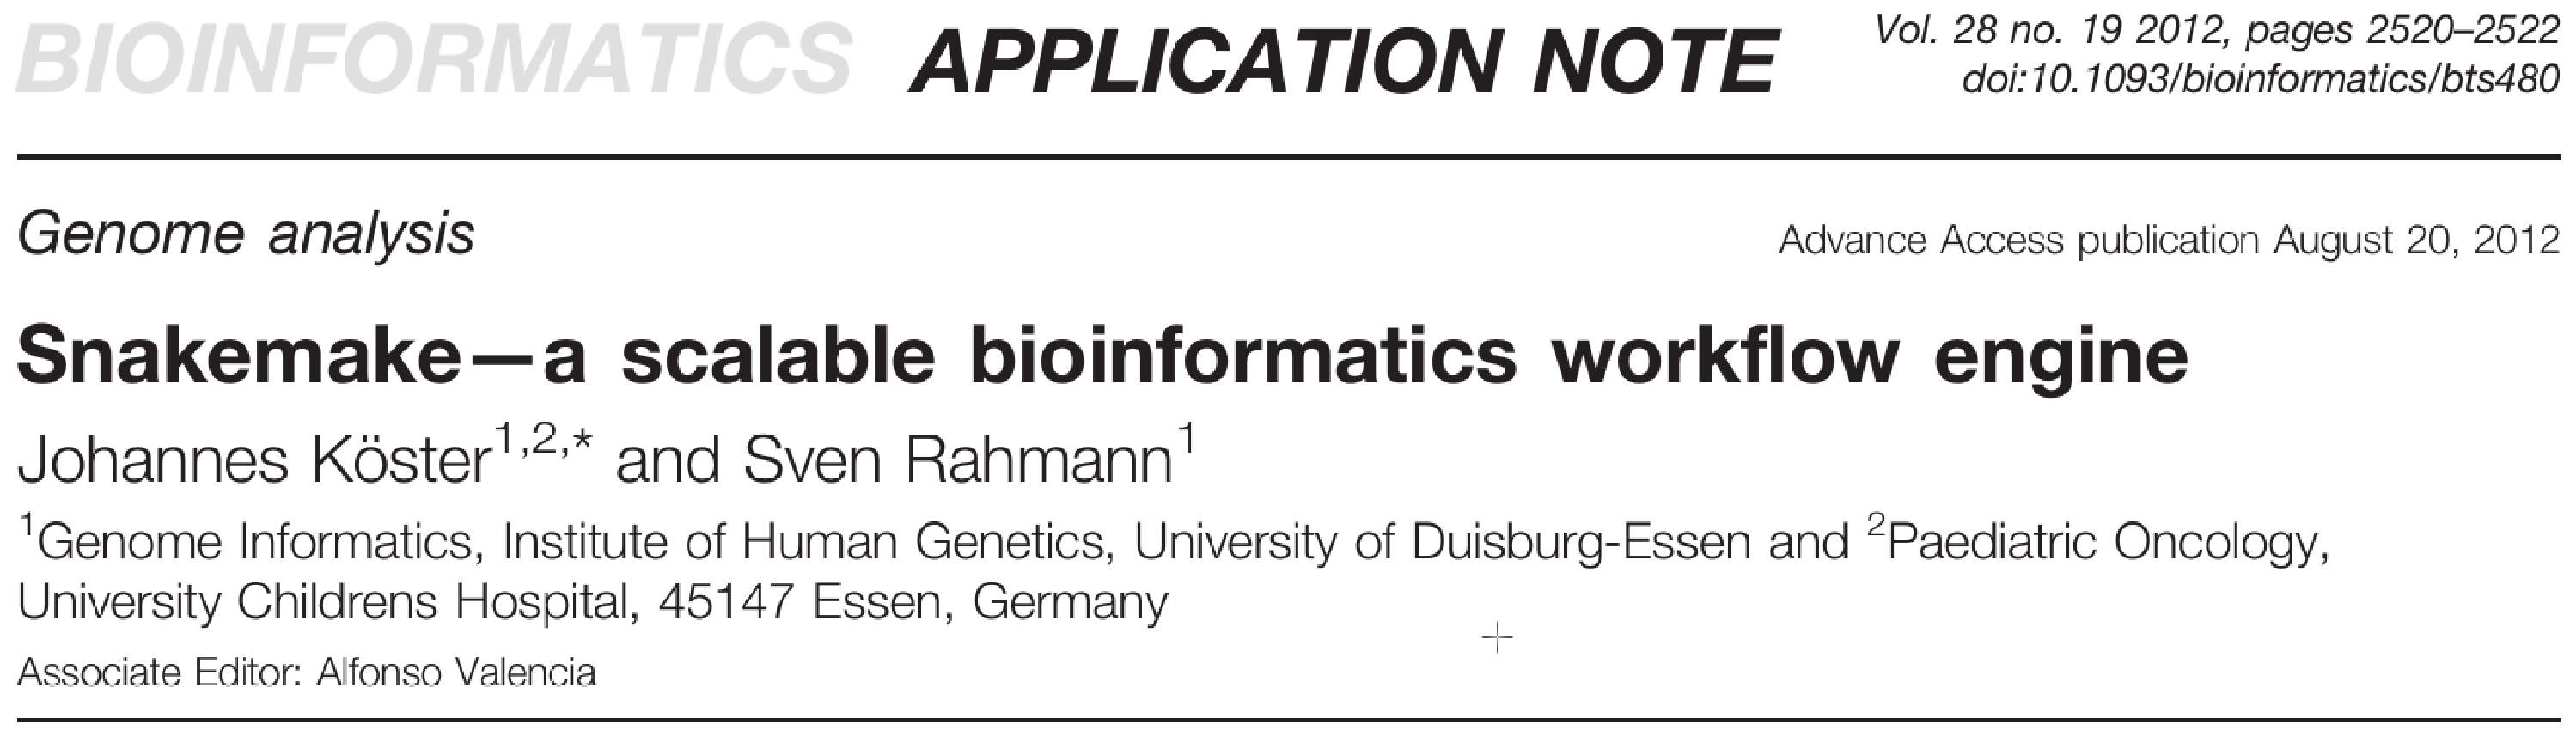
\includegraphics[width=\linewidth]{imgs/kr12-bio-cover}
\end{figure}

This (unfortunately) undersells it since users who want to do what Make does, would appreciate its Python-based syntax.

\end{frame}


